\section{Lead-Lag}

Un système Lead-Lag contient deux constantes de temps $T_{LEAD}$ et $T_{LAG}$, respectivement au numérateur et au dénominateur. Il peut avoir un certain gain statique $K_P$ et un délai $\theta$.
\begin{equation}
    P(s) = K_P \, \frac{T_{LEAD} s + 1}{T_{LAG} s + 1} \, e^{-\theta s}
\end{equation}
La valeur initiale du gain peut se calculer, et fait apparaître 3 scénarios : $T_{LEAD} < 0$, $T_{LEAD} > 0$ avec $T_{LEAD} > T_{LAG}$, ainsi que $T_{LEAD} > 0$ avec $T_{LEAD} < T_{LAG}$.
\begin{equation}
    y(0) = \lim_{s \to \infty} K_P \, \frac{T_{LEAD} s + 1}{T_{LAG} s + 1} \, e^{-\theta s} = K_P \, \frac{T_{LEAD}}{T_{LAG}}
\end{equation}
\begin{figure}[H]
    \centering
    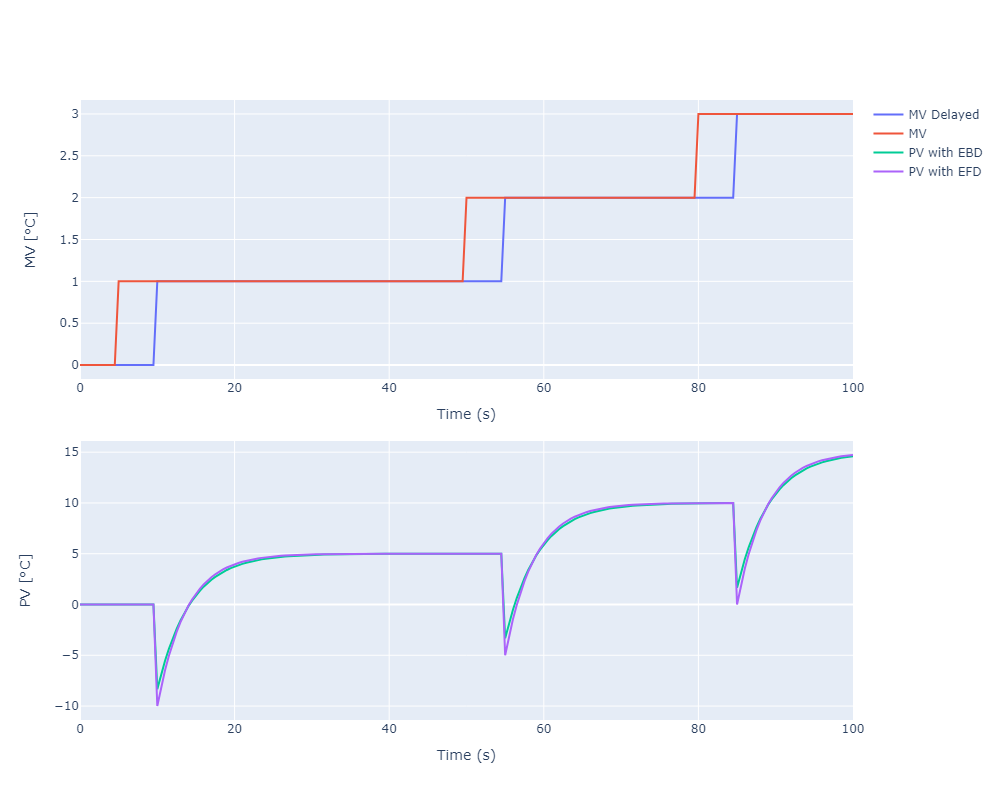
\includegraphics[width=0.8\textwidth]{../Plots/Lead-Lag/LL_Lead_negative.png}
    \caption{Réponse d'un système Lead-Lag avec $T_{LEAD} < 0$}
    \label{fig:Tlead_neg}
\end{figure}
Nous pouvons ici observer sur la Figure \ref{fig:Tlead_neg} le pic négatif dù à la constante Lead négative.
Il met ensuite un certain temps d'établissement pour atteindre le gain statique $K_P = 5$.
Le délai est également visible en voyant que $PV$ commence à agir après le délai appliqué sur $MV$.
Nous voyons de plus, que les méthodes EBD et EFD sont similaires en termes d'approximation, mais afin d'éviter les problèmes de stabilité du EFD, il est préférable d'utiliser EBD.
\begin{figure}[H]
    \centering
    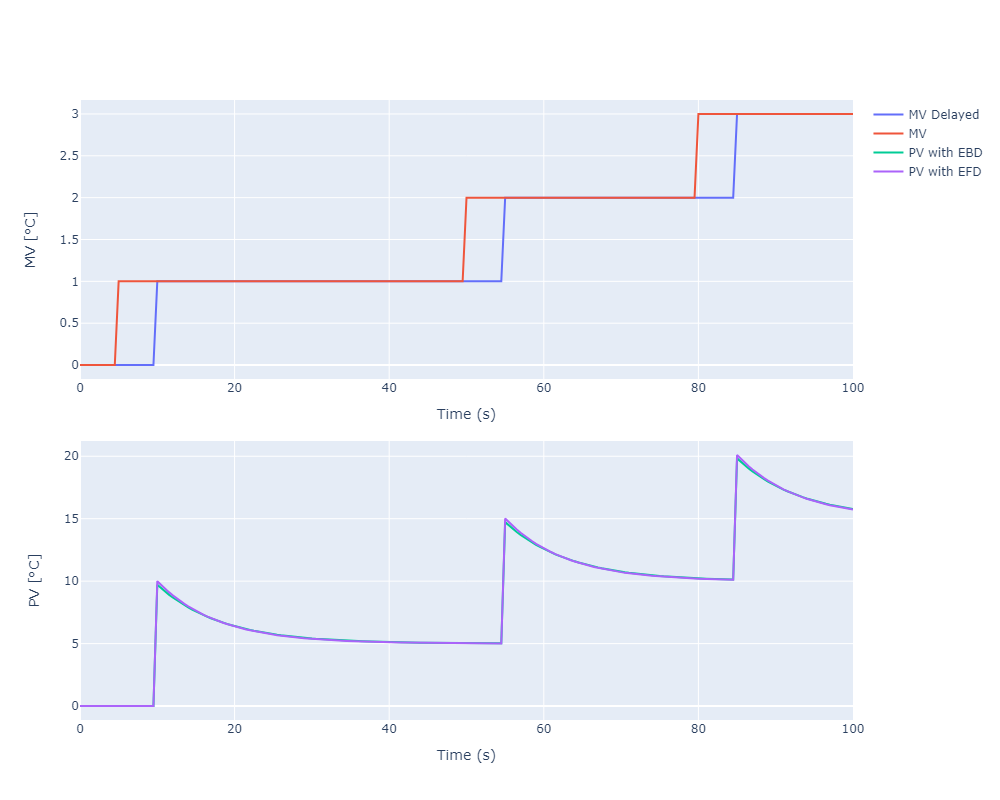
\includegraphics[width=0.8\textwidth]{../Plots/Lead-Lag/LL_Lead_higher_than_Lag.png}
    \caption{Réponse d'un système Lead-Lag avec $T_{LEAD} > T_{LAG} > 0$}
    \label{fig:Tlead_pos_Tlag_smaller}
\end{figure}
Dans le cas où $T_{LEAD} > T_{LAG}$, nous pouvons observer sur la Figure \ref{fig:Tlead_pos_Tlag_smaller} que le pic est bien positif et à une valeur double du gain statique puisque $T_{LEAD} = 2 \, T_{LAG}$.
\begin{figure}[H]
    \centering
    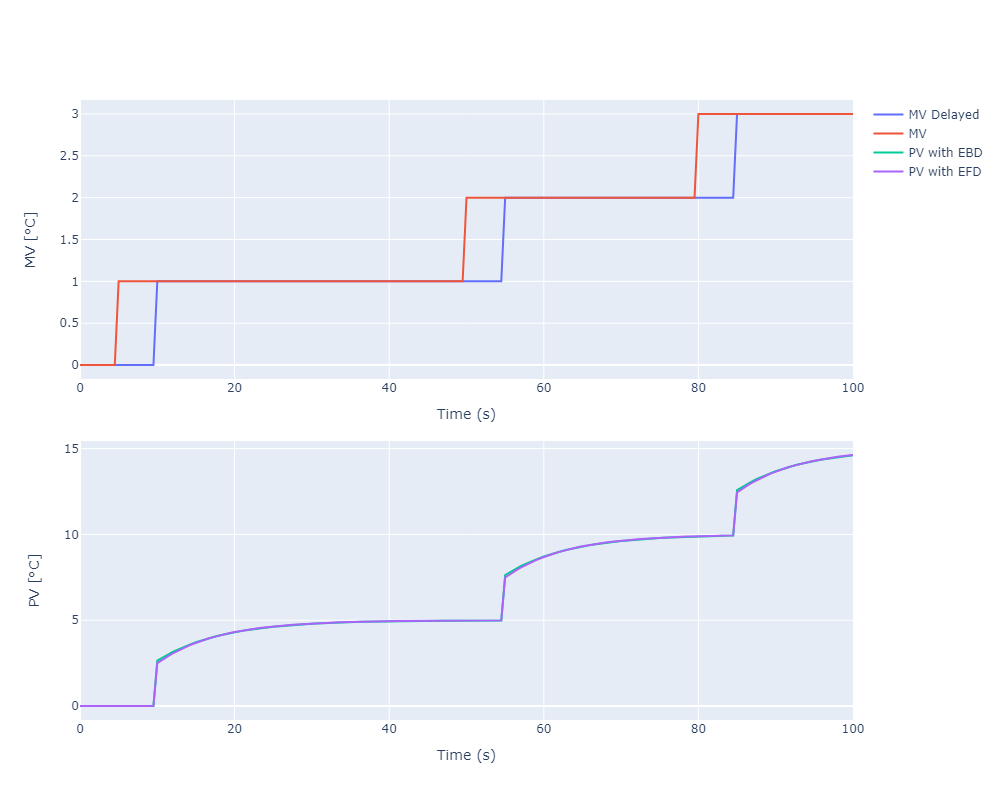
\includegraphics[width=0.8\textwidth]{../Plots/Lead-Lag/LL_Lead_lower_than_Lag.png}
    \caption{Réponse d'un système Lead-Lag avec $T_{LAG} > T_{LEAD} > 0$}
    \label{fig:Tlead_pos_Tlag_higher}
\end{figure}
Enfin, la Figure \ref{fig:Tlead_pos_Tlag_higher} montre le cas où $T_{LEAD} < T_{LAG}$, où le gain initial est 2 fois plus petit que le gain statique puisque $T_{LEAD} = 1/2 \, T_{LAG}$.